
\section{Zusammenfassung}
\label{sec:zusammenfassung}

\todo[inline, color=green]{Jan}


\section{Einleitung}
\label{sec:einleitung}

\todo[inline, color=green]{Jan}


\subsection{Kontext/Hintergrund}


\subsection{Projekt Motivation}


\subsection{Problemstellung}


\subsection{Projektziele}


\subsection{Projektumfang}


\subsection{Übersicht über die Dokumentation}


\section{Methodik}
\label{sec:methodik}

\todo[inline, color=green]{Simon}


\section{Software und User Interface}
\label{sec:software_und_user_interface}

\todo[inline, color=green]{Leopold}


\subsection{Messsoftware}
\label{subsec:messsoftware}

Die Messsoftware dieses Projekts setzt sich aus mehreren Programmen zusammen.
Die genaue Funktionsweise und Interaktionen der einzelnen Programme miteinander werden nun im Folgenden erklärt.


\subsection{Datenbanksystem}
\label{subsec:datenbanksystem}


\subsubsection{Einführung}

Das Datenbanksystem (DBS) wurde ursprünglich mit SQLite3 implementiert, da es relativ einfach und intuitiv zu handhaben ist benutz haben wir eine SQL Row based Datenbank. Allerdings ergeben sich hierbei Probleme bei mehrfachen Zugriffen auf die Datenbank. Um diese Herausforderungen zu lösen, wurde auf ein Server-Client-Modell mit PostgreSQL umgestellt.


\subsubsection{Problemstellung bei SQLite3}

SQLite3 basiert auf Binärcode, was zu Problemen führen kann, wenn zwei Anwendungen gleichzeitig auf die gleiche Datenbank zugreifen. In diesem Szenario schreibt das Prozessprogramm (Python) die Messwerte in die Datenbank, während die GUI (Webapplikation) die Daten aus der Datenbank liest. Wenn das Prozessprogramm gerade Daten in die Datenbank schreibt, wird diese blockiert. Dadurch kann nicht gleichzeitig aus der Datenbank gelesen werden.


\subsubsection{Lösung: Umstellung auf PostgreSQL}

Um die gleichzeitige Nutzung durch mehrere Anwendungen zu ermöglichen, wurde auf PostgreSQL umgestellt. Als Open-Source-Datenbank bietet PostgreSQL folgende Vorteile:

\begin{itemize}
    \item Multi-User-Unterstützung: Mehrere Clients können gleichzeitig auf den zentralen Server zugreifen.
    \item Transaktionssicherheit: Durch den Einsatz von Transaktionen werden Schreib- und Lesevorgänge konsistent und sicher abgewickelt.
    \item Erweiterbarkeit: Zahlreiche Erweiterungen und Anpassungsmöglichkeiten machen PostgreSQL zu einer flexiblen Lösung.
    \item Netzwerkbasierter Zugriff: Das System kann als zentraler Datenbankserver in unterschiedlichen Umgebungen eingesetzt werden.
\end{itemize}

Aktuell läuft der PostgreSQL-Server auf einem Raspberry Pi. Eine zukünftige Weiterentwicklung sieht jedoch den Betrieb auf einem zentralen Server vor, wobei einzelne Komponenten wie die grafische Benutzeroberfläche (GUI) ebenfalls ausgelagert werden könnten.


\subsubsection{Schematischer Aufbau}
\label{subsubsec:schematischer_aufbau}

\begin{figure}[h]
	\centering
	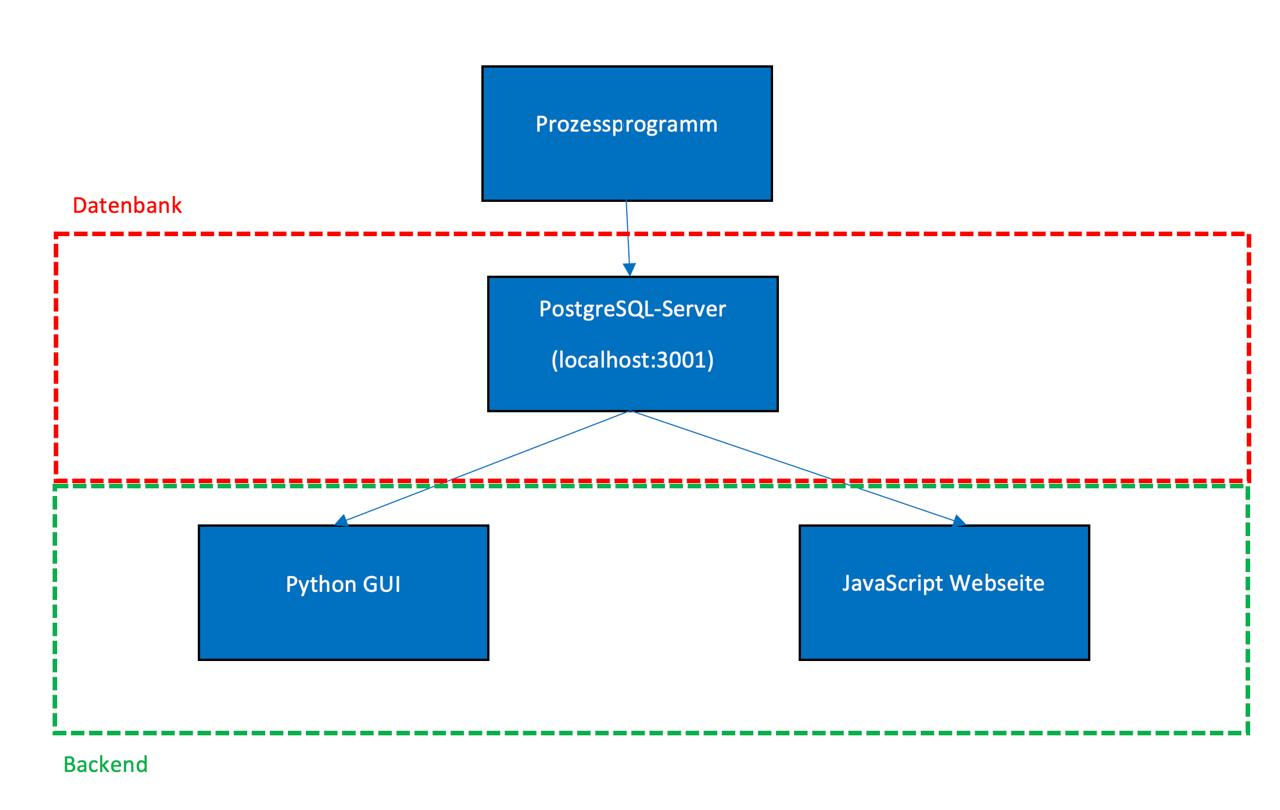
\includegraphics[width=0.4\linewidth]{figures/Schematischer Aufbau.jpeg}
	\caption[Schematischer Aufbau]{Schematischer Aufbau des Datenbanksystems}\label{fig:schematischer_aufbau}
\end{figure}
\todo{Bildgröße am Ende anpassen}


\subsubsection{Zusammenfassung}
\label{subsubsec:zusammenfassung}

Durch PostgreSQL wird ein robustes und flexibles Datenbanksystem geschaffen, das die Vorteile beider Technologien vereint. Das Frontend in Python erlaubt eine lokale Steuerung, während die Website als Verwaltungspunkt für einen Admin dient. Insgesamt lässt sich das System als lehr- und praxisnah bewerten.


\subsection{Technologien und Architektur}
\label{subsec:technologien_und_architektur}


Für die Umsetzung der Webanwendung haben wir uns für einen aktuellen Technologie-Stack entschieden, der uns viel Flexibilität und eine klare Struktur bietet:

\begin{itemize}
    \item \textbf{HTML5 \& CSS3:}\newline Die Grundstruktur der Anwendung basiert auf HTML5. Für das Styling nutzen wir CSS3 in Kombination mit Tailwind CSS, was uns ein responsives und ansprechendes Design ermöglicht.
    \item \textbf{JavaScript \& Chart.js:}\newline Dynamische Inhalte und interaktive Elemente werden mit JavaScript realisiert. Für die Darstellung von Diagrammen, etwa zur Visualisierung von Temperaturverteilungen oder Mitarbeiterrollen, setzen wir auf Chart.js.
    \item \textbf{RESTful API:}\newline Um eine reibungslose Kommunikation zwischen Frontend und Backend sicherzustellen, verwenden wir eine RESTful API, die im JSON-Format arbeitet. Über diese Schnittstelle werden Funktionen wie die Benutzerregistrierung, der Login, die Mitarbeiterverwaltung und diverse Datenbankabfragen abgewickelt.
    \item \textbf{Responsive Design:}\newline Dank moderner CSS-Frameworks und responsiven Layouts passt sich die Anwendung automatisch an verschiedene Geräte an – egal, ob auf dem Desktop oder auf mobilen Geräten.
\end{itemize}


\subsection{Benutzerinterface und Funktionalitäten}
\label{subsec:benutzerinterface_und_funktionalitäten}

Das Benutzerinterface ist in mehrere Bereiche unterteilt, um die Bedienung möglichst einfach zu gestalten. 

\begin{figure}[h]
	\centering
	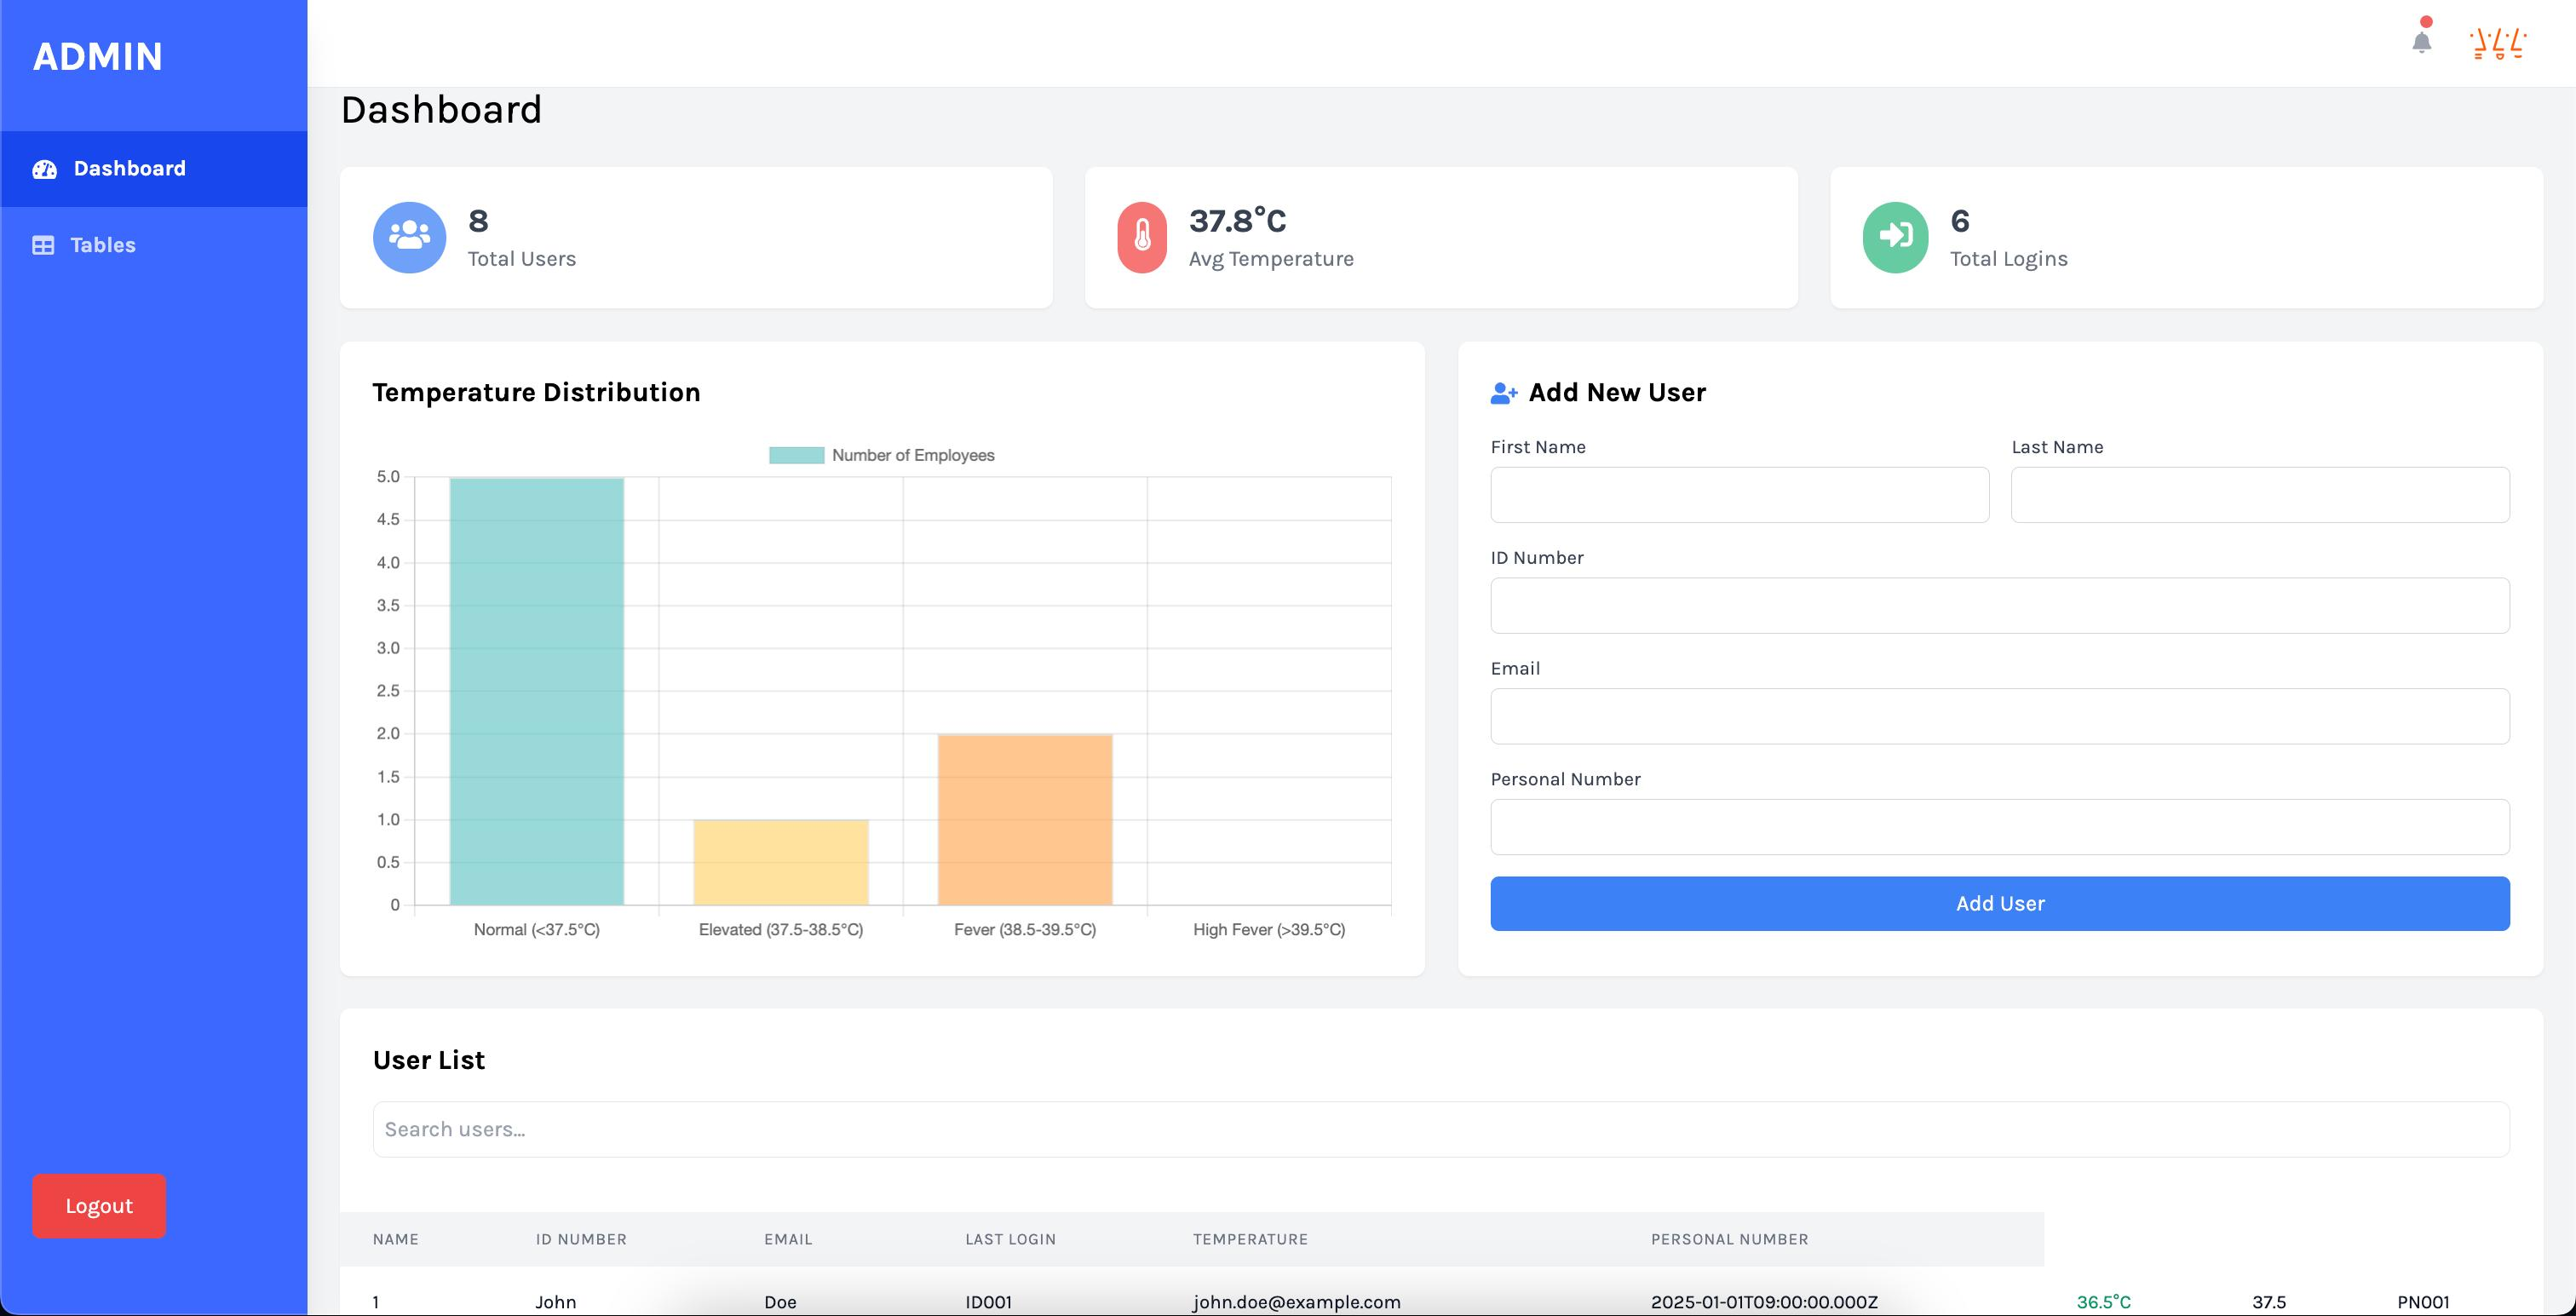
\includegraphics[width=0.4\linewidth]{figures/GUI.jpeg}
	\caption[GUI]{Ausschnitt aus dem Graphical User Interface (GUI)}\label{fig:gui}
\end{figure}
\todo{Bildgröße am Ende anpassen}

Über eine ständig sichtbare Sidebar mit passenden Icons gelangt man schnell zu wichtigen Bereichen wie dem Dashboard oder den Tabellenansichten. Im Dashboard bekommt man einen Überblick über wichtige Kennzahlen – etwa die Anzahl der Nutzer, die Durchschnittstemperatur und die Login-Aktivitäten – die in Echtzeit aktualisiert werden. 

\vspace{1em}
\noindent Neue Benutzer oder Mitarbeiter können über das Login hinzugefügt werden, wobei Eingaben sofort validiert werden und Fehler direkt angezeigt werden. 

\vspace{1em}
\noindent Die Messdaten werden übersichtlich in Diagrammen dargestellt, zum Beispiel zeigt ein Balkendiagramm die Temperaturverteilung und ein anderes Diagramm die Verteilung der Mitarbeiterrollen.

\vspace{1em}
\noindent Zudem sorgen Such- und Filterfunktionen in den Tabellen dafür, dass man die Daten schnell durchsuchen und analysieren kann. Die Anmeldung erfolgt über ein Login-System, das auf JSON Web Tokens (JWT) basiert, sodass nur berechtigte Nutzer Zugriff auf die Anwendung haben.

\vspace{1em}
\noindent\textbf{Fazit:}\newline
Durch die Kombination dieser Technologien entstand eine benutzerfreundliche Webanwendung, die alle wichtigen Daten zentral anzeigt und verwaltet. Die modulare Architektur erlaubt zudem eine einfache Erweiterung, falls zukünftig weitere Anpassungen notwendig werden falls unser Projekt jemals in Produktion gehen würde.


\subsection{API-Dokumentation}
\label{subsec:api-dokumentation}

Die API unterstützt die Benutzer- und Mitarbeiterverwaltung sowie die Kommunikation mit der Datenbank. Im Folgenden sind die wichtigsten Endpunkte und deren Funktion kurz zusammengefasst.


\subsubsection{Allgemeines}

\begin{itemize}
    \item \textbf{Datenformat: }Alle Anfragen und Antworten erfolgen in JSON.
    \item \textbf{Fehler: }Bei ungültigen Anfragen wird eine entsprechende Fehlermeldung mit HTTP-Statuscode zurückgegeben.
    \item \textbf{Port: }Standardmäßig läuft der Server auf Port 3001 (konfigurierbar über .env).
\end{itemize}


\subsubsection{Benutzerverwaltung}

\textbf{Registrierung}
\begin{itemize}
    \item \textbf{Methode: }POST 
    \item \textbf{Endpoint: }/api/register 
    \item \textbf{Body: } \begin{minted}[linenos]{JSON}
{
  "username": "testuser",
  "password": "securepassword"
}
    \end{minted}
    \item \textbf{Antworten: }
    \begin{itemize}
        \item \textit{201 Created: }Benutzer erfolgreich registriert
        \item \textit{400 Bad Request: }Benutzername existiert bereits oder erforderliche Felder fehlen
        \item \textit{500 Internal Server Error: }Fehler beim Speichern in der Datenbank
    \end{itemize}
\end{itemize}
%\todo{Code noch besser formatieren}
\textbf{Login}
\begin{itemize}
    \item \textbf{Methode: }POST 
    \item \textbf{Endpoint: }/api/login  
    \item \textbf{Body: } \begin{minted}[linenos]{JSON}
{
  "username": "testuser",
  "password": "securepassword"
}
    \end{minted}
    \item \textbf{Antworten: }
    \begin{itemize}
        \item \textit{200 OK: }Login erfolgreich, liefert ein JWT-Token (gültig für eine Stunde)
        \item \textit{401 Unauthorized: }Falscher Benutzername oder Passwort
        \item \textit{500 Internal Server Error: }Fehler beim Abrufen des Benutzers
    \end{itemize}
\end{itemize}


\subsubsection{Datenbankverwaltung}

\textbf{Datenbankverbindung testen}
\begin{itemize}
    \item \textbf{Methode: }GET 
    \item \textbf{Endpoint: }/test-db
    \item \textbf{Antworten: }
    \begin{itemize}
        \item \textit{200 OK: }Verbindung erfolgreich
        \item \textit{500 Internal Server Error: }Fehlerhafte Verbindung
    \end{itemize}
\end{itemize}


\subsubsection{Mitarbeiterverwaltung}

\textbf{Mitarbeiter abrufen}
\begin{itemize}
    \item \textbf{Methode: }GET 
    \item \textbf{Endpoint: }/api/employees
    \item \textbf{Antworten: }
    \begin{itemize}
        \item \textit{200 OK: }Array mit allen Mitarbeitern
        \item \textit{500 Internal Server Error: }Fehler beim Abrufen der Daten
    \end{itemize}
\end{itemize}

\textbf{Neuen Mitarbeiter hinzufügen}
\begin{itemize}
    \item \textbf{Methode: }POST 
    \item \textbf{Endpoint: }/api/employess  
    \item \textbf{Body: } \begin{minted}[linenos]{JSON}
{
    "first_name": "Max",
    "last_name": "Mustermann",
    "id_number": "12345",
    "email": "max@example.com",
    "personal_number": "67890"
}
    \end{minted}
    \item \textbf{Antworten: }
    \begin{itemize}
        \item \textit{201 Created: }Mitarbeiter erfolgreich gespeichert
        \item \textit{400 Bad Request: }Fehlende oder ungültige Felder
        \item \textit{500 Internal Server Error: }Fehler beim Speichern des Mitarbeiters
    \end{itemize}
\end{itemize}


\section{Ergebnisse und Diskussion}
\label{sec:ergebnisse_und_diskussion}

\todo[inline, color=green]{Janis}


\section{Fazit und Ausblick}
\label{sec:fazit_und_ausblick}


\subsection{Zusammenfassung der Arbeit}

\todo[inline, color=green]{Janis}


\subsection{Diskussion der Implikationen}

\todo[inline, color=green]{Leopold}
Unsere Untersuchung hat wesentlich dazu beigetragen, grundlegende Zusammenhänge in der Informatik und Elektrotechnik besser zu verstehen. Besonders hervorzuheben ist dabei die Anwendung eines webbasierten Systems welches in Zusammenhang mit einem lokalen Prototyp zusammenspielt. Die PostgreSQL Datenbank könnte durch Zukunftssicherheit auch direkt in Produktion deployt werden. Dasselbe gilt (mit Ausnahme der Authentizität) auch für die Webanwendung.

\vspace{1em}
\noindent Besonders positiv ist, dass die benutzerfreundliche GUI, die auf mobilen Geräten nutzbar ist, zeigt, wie technische Messungen auch für Laien verständlich aufbereitet werden können. Dies fördert nicht nur den Alltagseinsatz neuer Technologien, sondern steigert auch das Bewusstsein für Energieeffizienz und Nachhaltigkeit.

\vspace{1em}
\noindent Insgesamt liefert das Projekt eine fundierte Basis für weiterführende Studien und Anwendungen, die dazu beitragen können, die die Gesundheit und Nachhaltigkeit von Mitarbeitern und Applikationen zu verbessern.


\subsection{Bereiche für zukünftige Arbeiten}

\todo[inline, color=green]{Janis}